\section{Вычислительные эксперименты}
    Исследуемая область является квадратом, размером 1 на 1. В качестве функции тока возьмём:
    \[
        \psi(x, y) = \sin (2 \pi x) \sin(\pi y),
    \]

    откуда получаем:
    \[
        \left\{
            \begin{split}
                & u(x, y) = -\pi \sin (2 \pi x) \cos(\pi y), \\
                & v(x, y) = 2\pi \cos (2 \pi x) \sin(\pi y).
            \end{split}
        \right.
    \]

    Изобразим фазовые кривые этой функции тока.
    \begin{figure}[H]
        \centering
        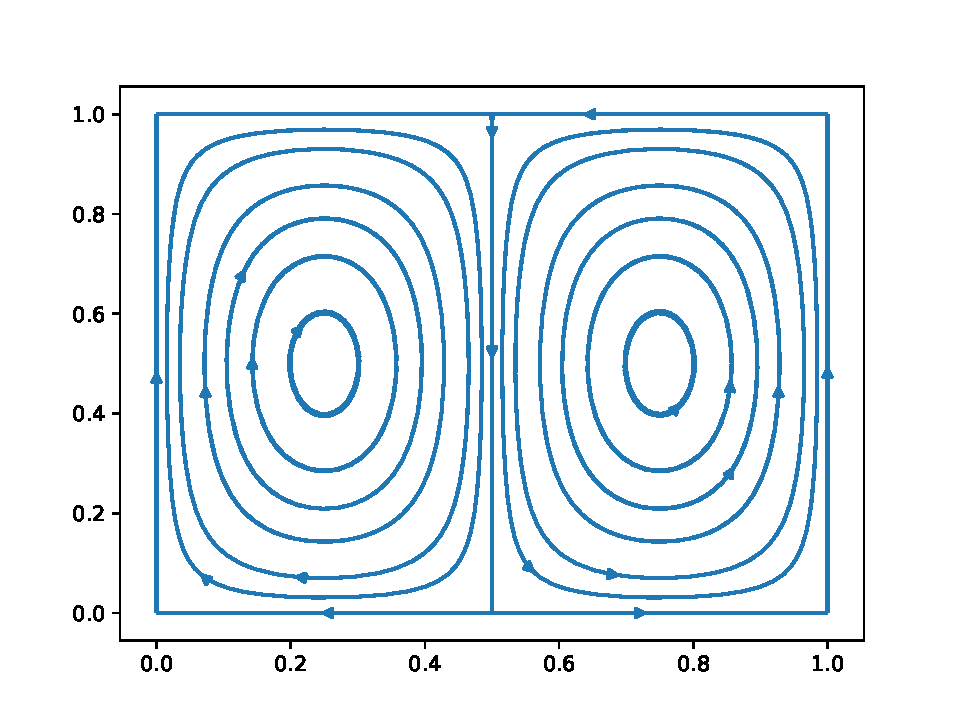
\includegraphics[width=8cm]{pictures/streamplot.pdf}
        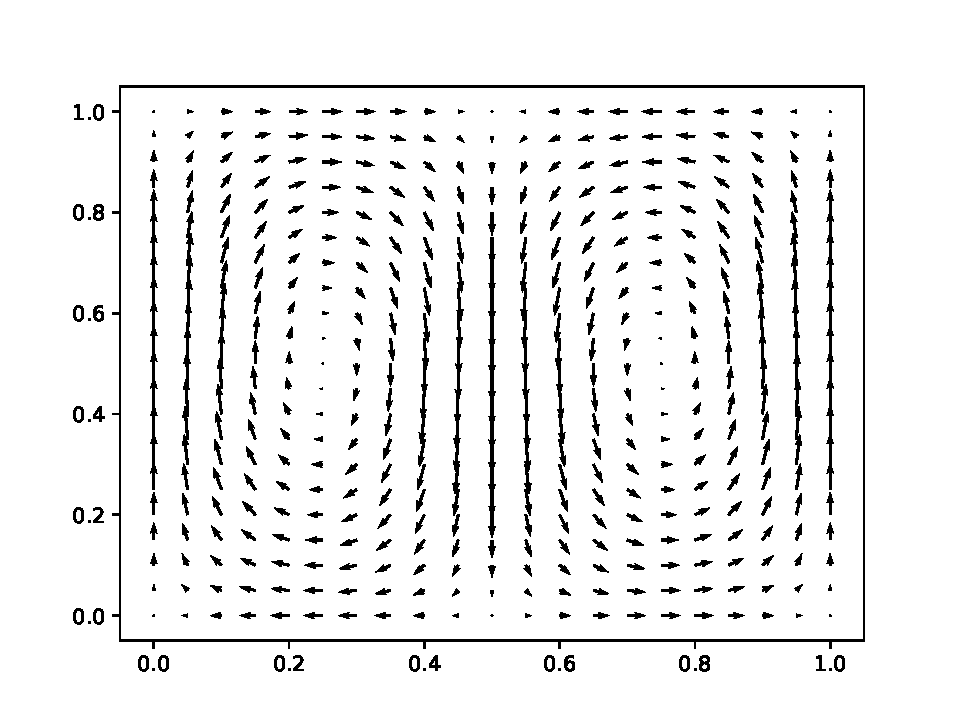
\includegraphics[width=8cm]{pictures/quiver.pdf}
        \caption{Фазовые кривые функции тока \( \psi(x, y) \).}
    \end{figure}

    В качестве начальной концентрации используем такую функцию:
    \[
        C_0(x, y) = \arctan \left( \frac{y - 0.5}{0.1} \right)
    \]

    \subsection{Алгоритм}
        Для реализации модели будем использовать конечно-разностный метод Рунге-Кутты 4 порядка. Для этого был использован язык Python с библиотеками numpy, matplotlib и scipy.

        Создадим в исследуемой области большое количество точек и для каждой из них применим метод на промежутке времени \( [0, 0.4] \). Выберем несколько моментов времени в которых построим все точки, а также интерполяционное изображение из этих точек.
        
        Интерполяция будет производиться методом линейной триангуляции, который реализуется встроенной функцией griddata.

    \subsection{Численный анализ}
        Для начала построим изображение пути трёх точек в данной области.
        \begin{figure}[H]
            \centering
            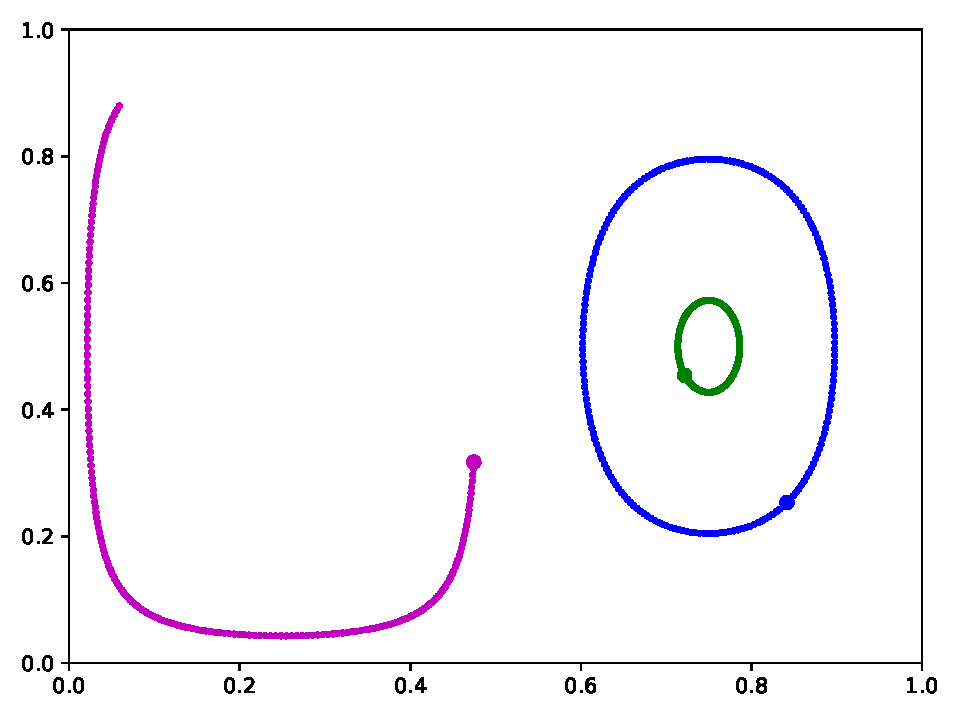
\includegraphics[width=12cm]{pictures/three.pdf}
        \end{figure}
        Эти пути следуют фазовым кривым, чего и следовало ожидать.

        Теперь рассмотрим поведение только одной центральной линии из 2000 точек на меньшем промежутке времени.  
        \begin{figure}[H]
            \centering
            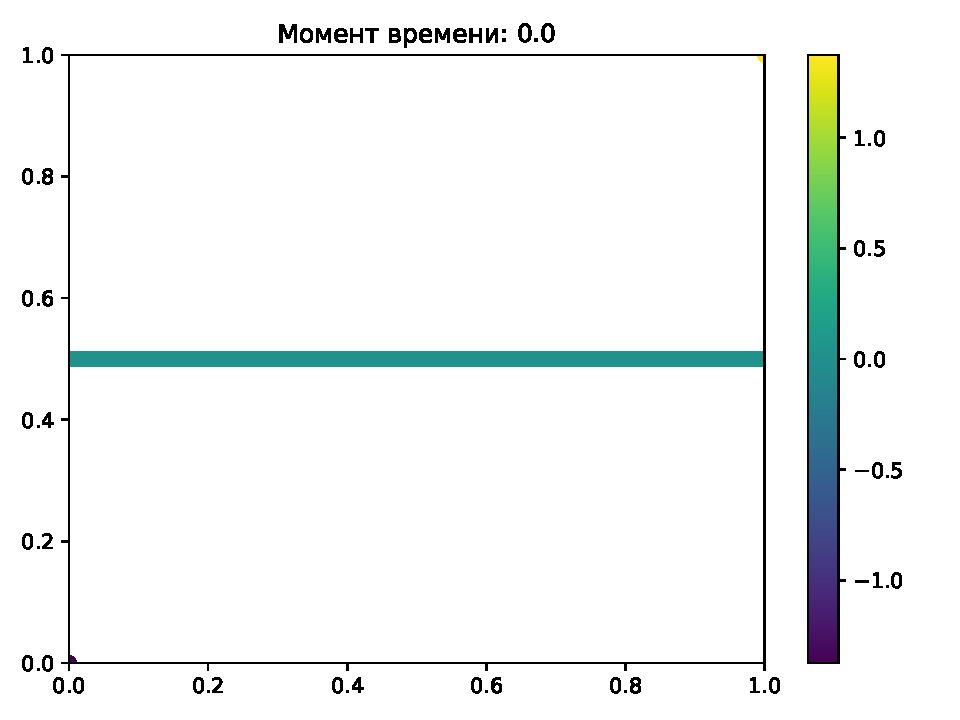
\includegraphics[width=8cm]{pictures/line0.pdf}
            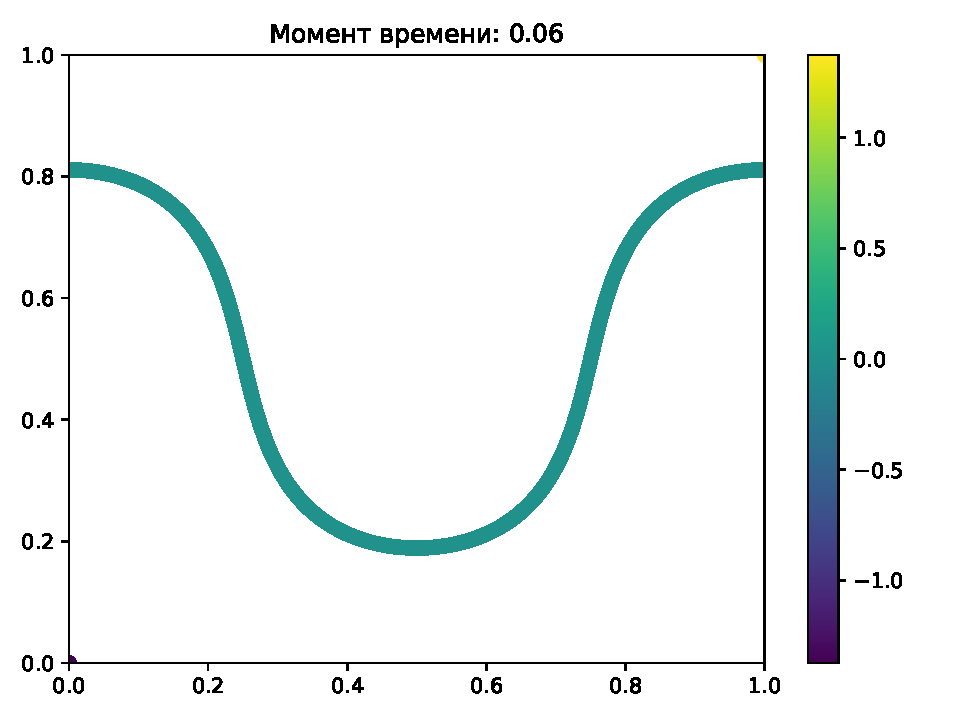
\includegraphics[width=8cm]{pictures/line3.pdf}
        \end{figure}
        \begin{figure}[H]
            \centering
            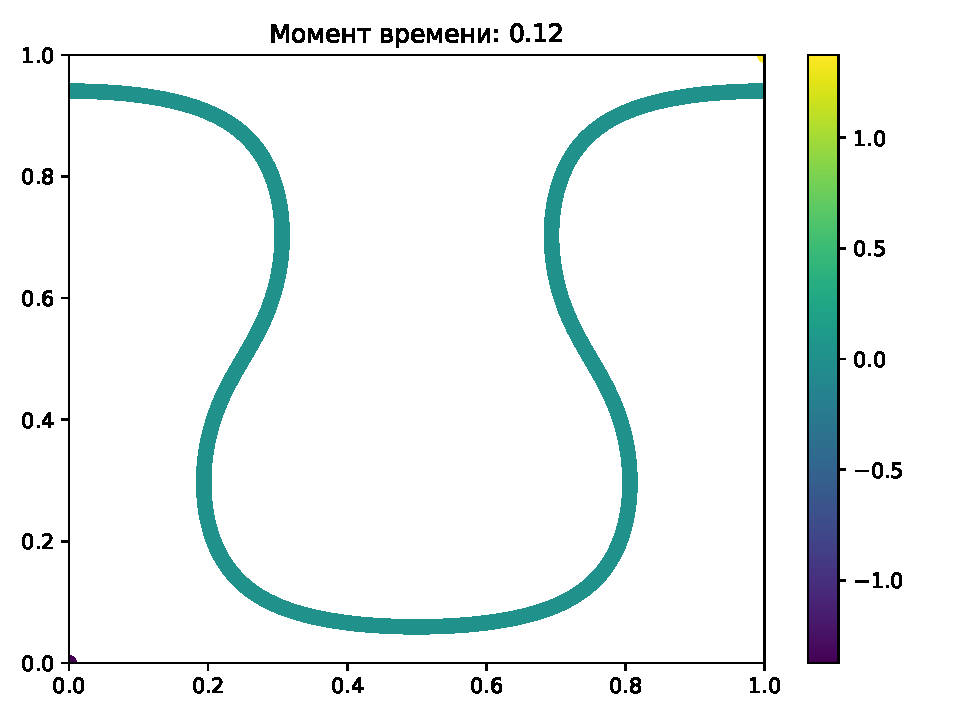
\includegraphics[width=8cm]{pictures/line6.pdf}
            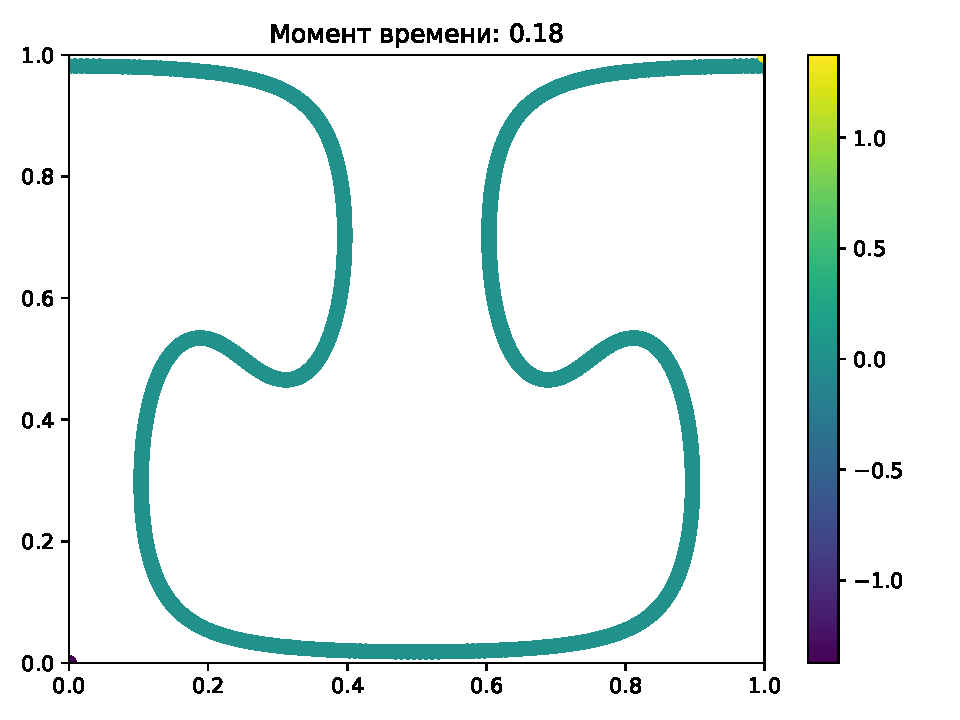
\includegraphics[width=8cm]{pictures/line9.pdf}
        \end{figure}

        На этом примере можно сделать предположения о поведении большого множества точек в данной области, например, образование изображения, похожего на гриб.


    \subsection{Результаты}
        Для получения результата на всей области построим 20000 случайных точек, после чего смоделируем их движение. После чего интерполируем на сетке, состоящей из 500 делений по обоим направлениям.

        Слева находится изображение со всеми точками, а справа интерполированное изображение в этот же момент времени.

    \begin{figure}[H]
        \centering
        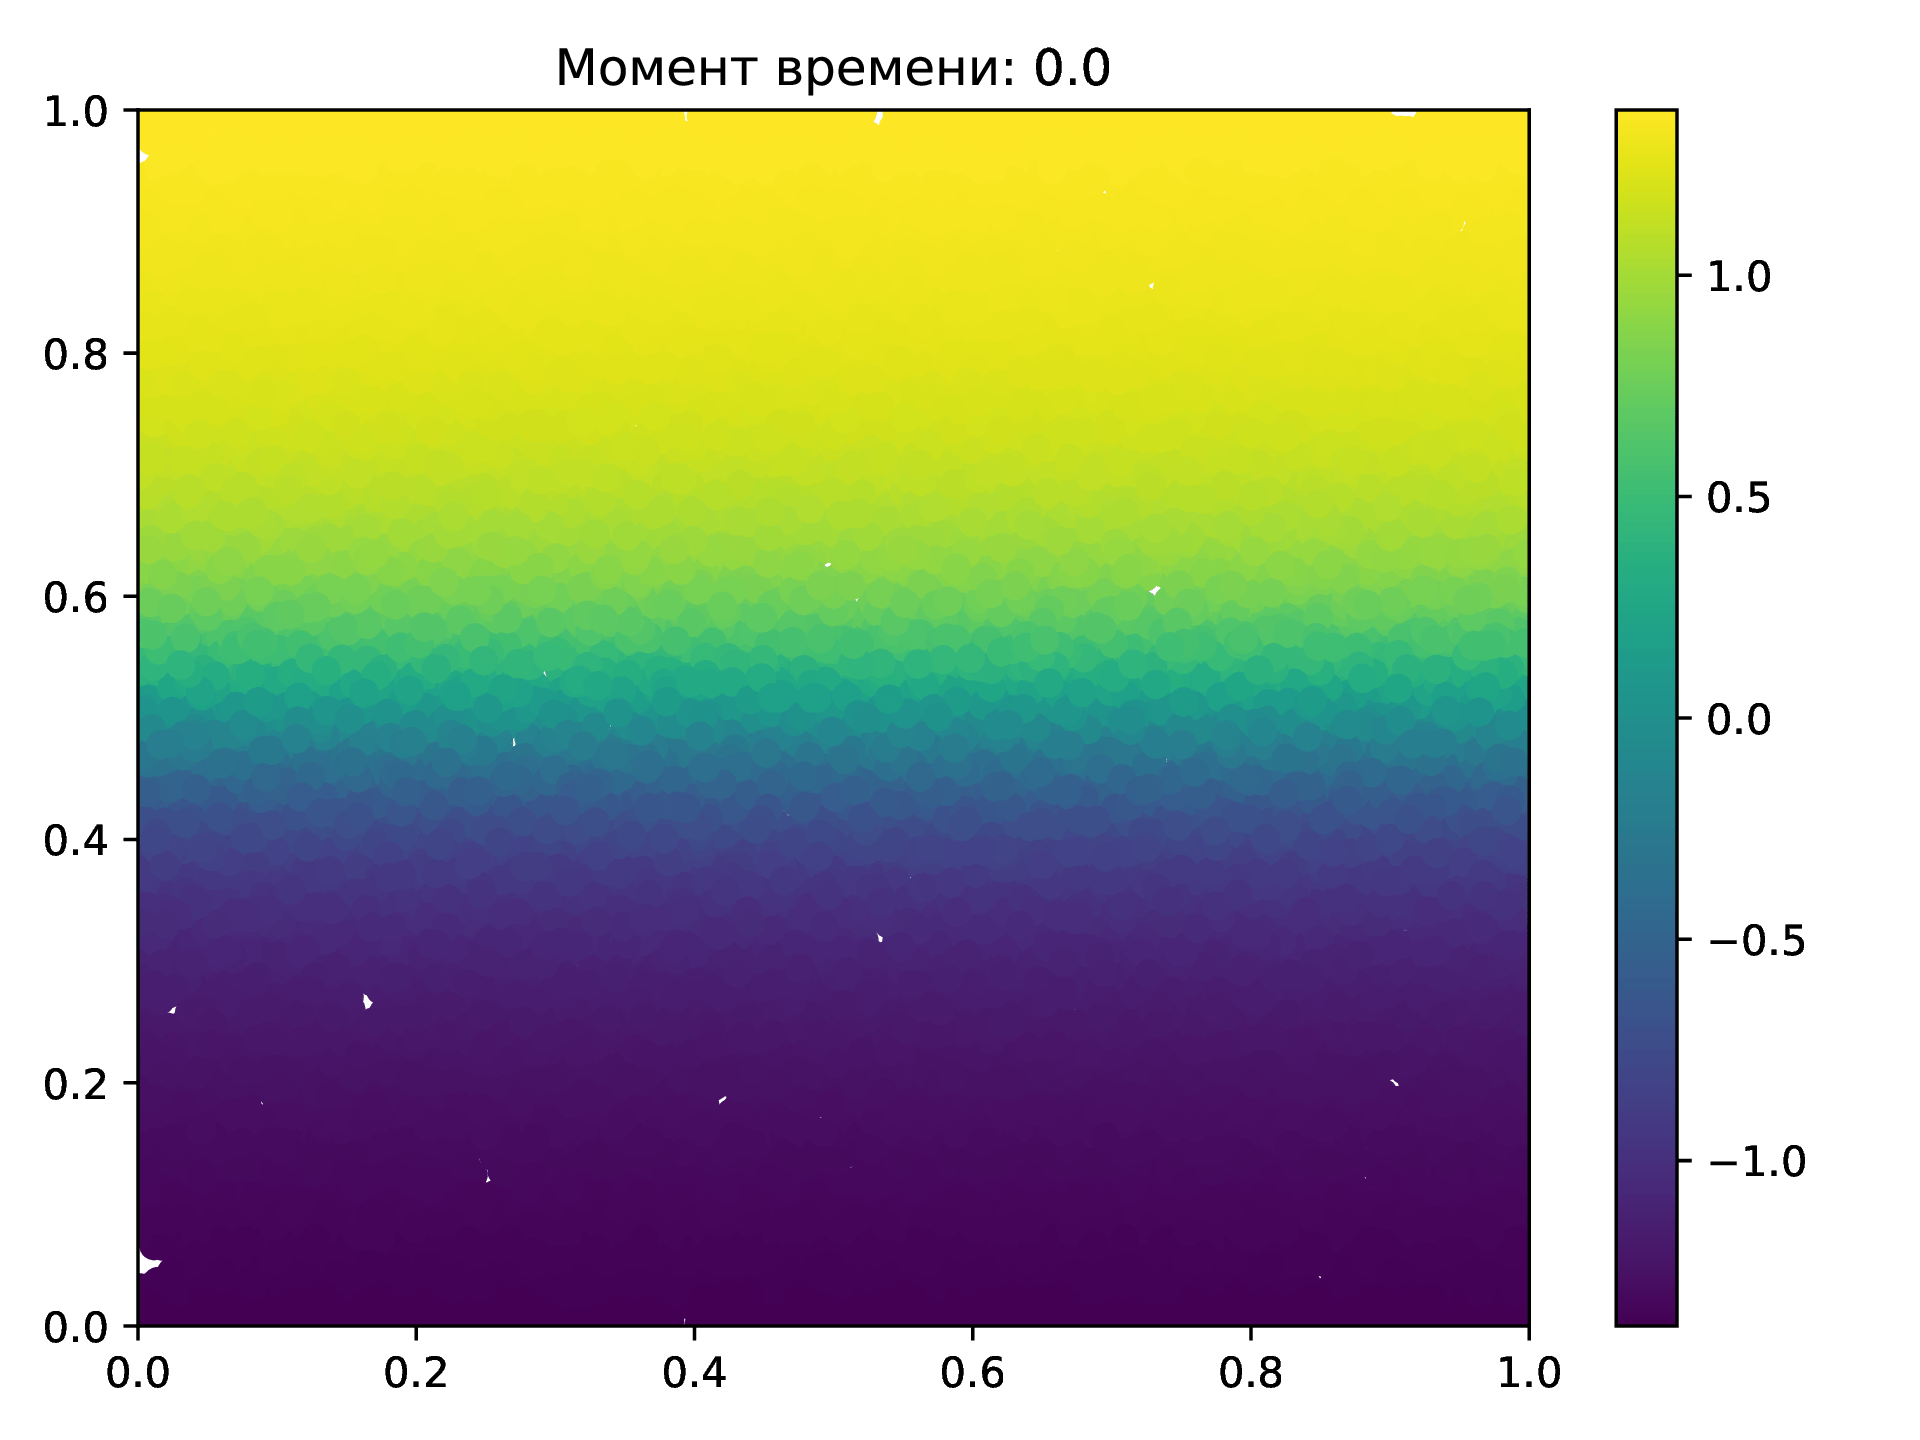
\includegraphics[width=8cm]{pictures/s0.png}
        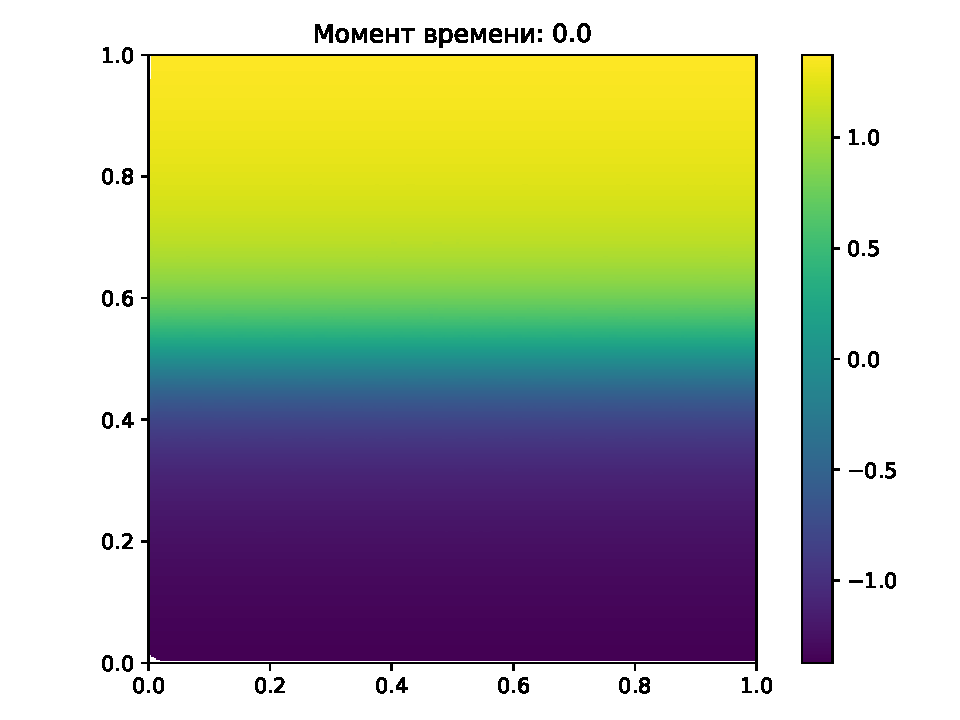
\includegraphics[width=8cm]{pictures/p0.pdf}
    \end{figure}
    \begin{figure}[H]
        \centering
        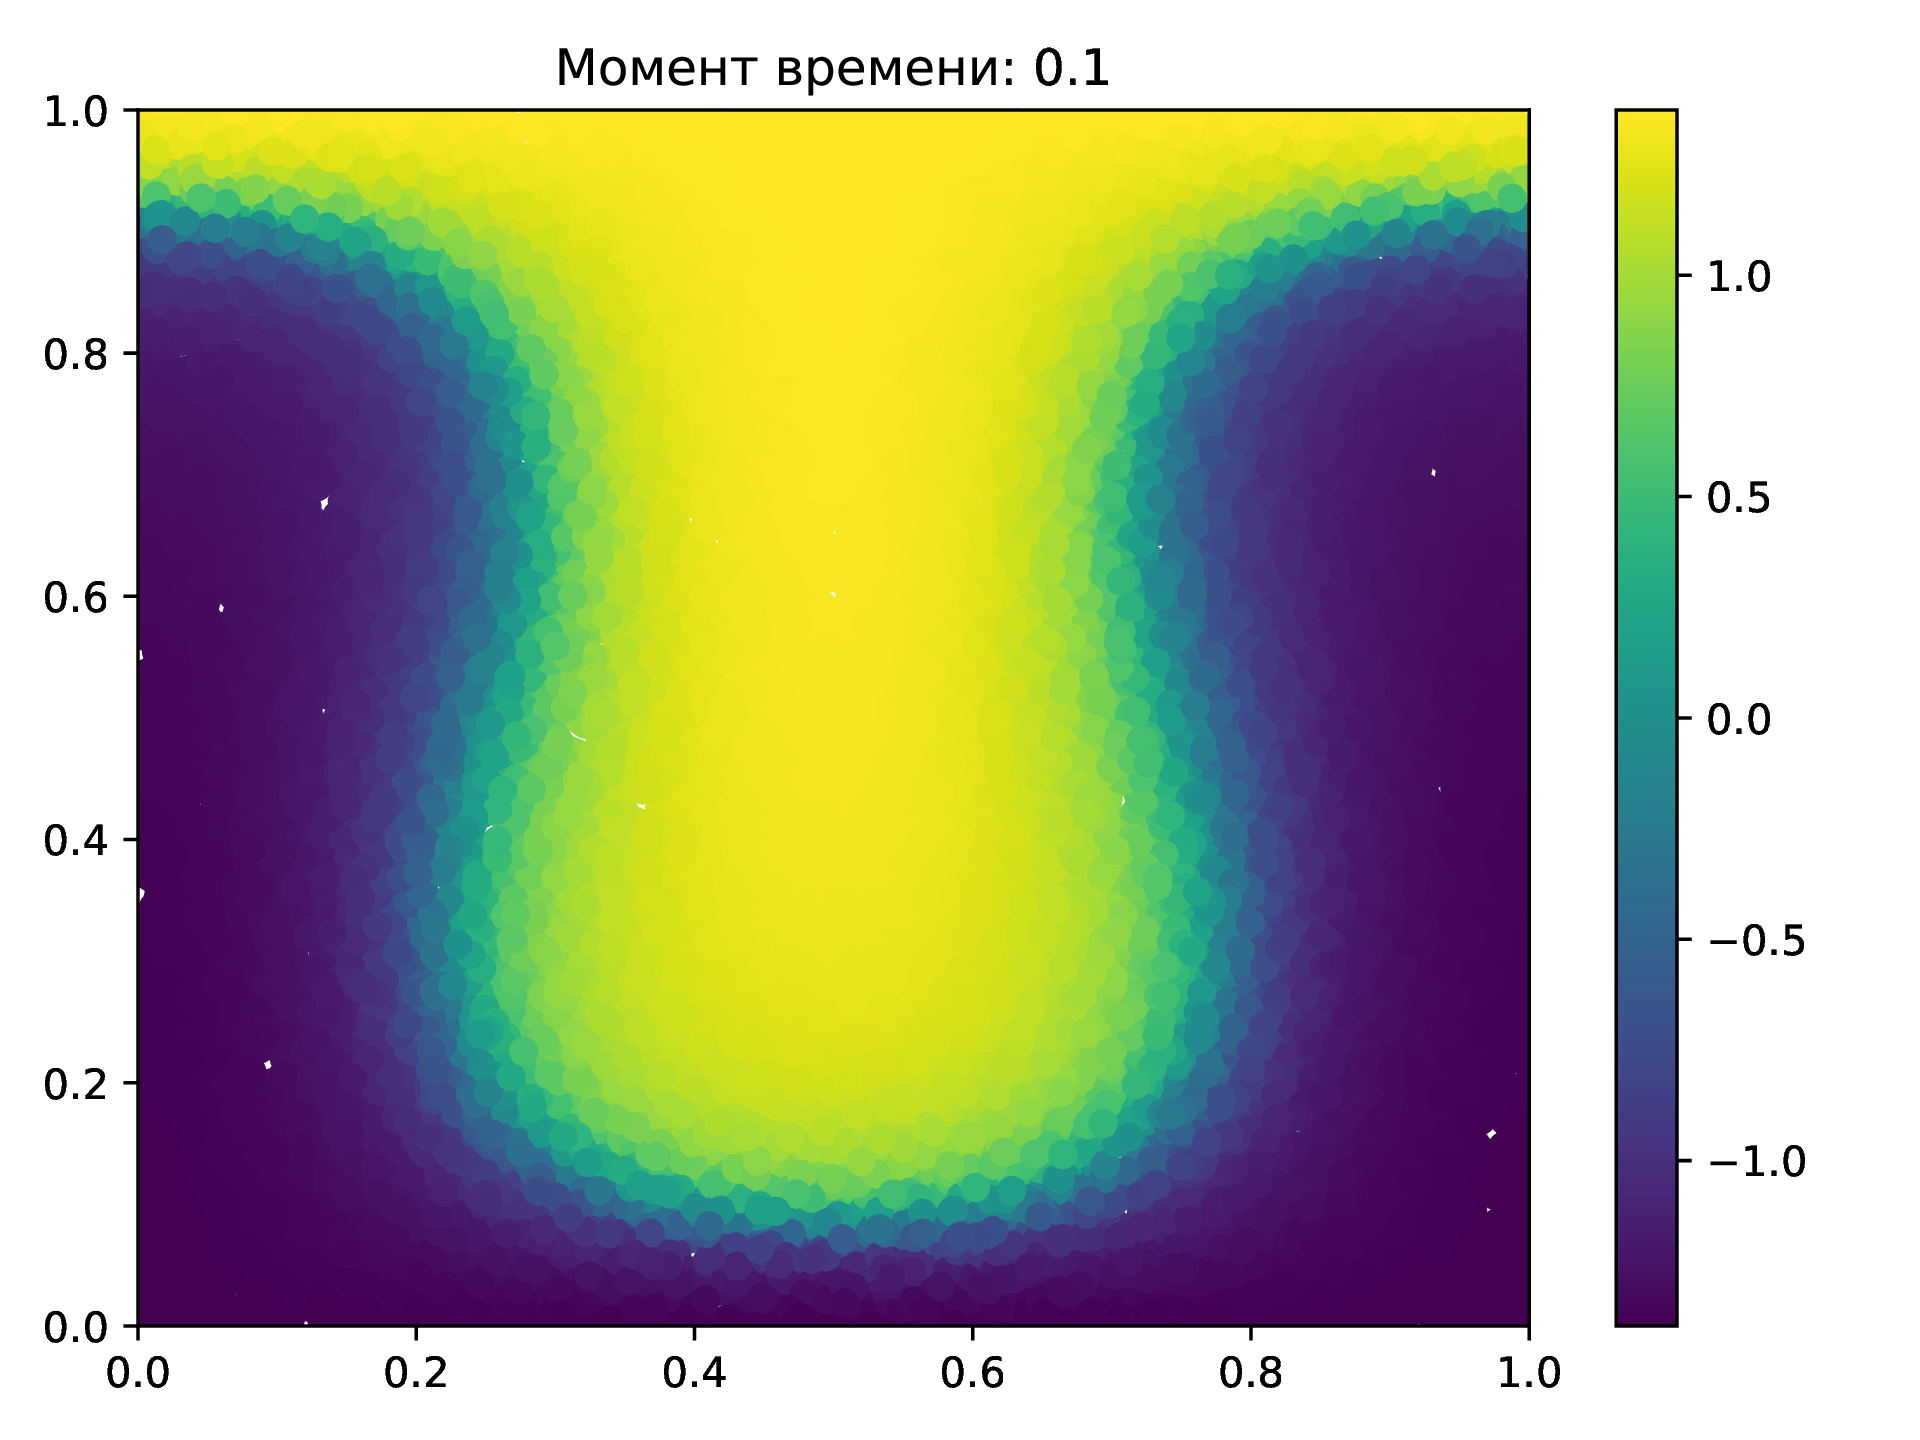
\includegraphics[width=8cm]{pictures/s5.png}
        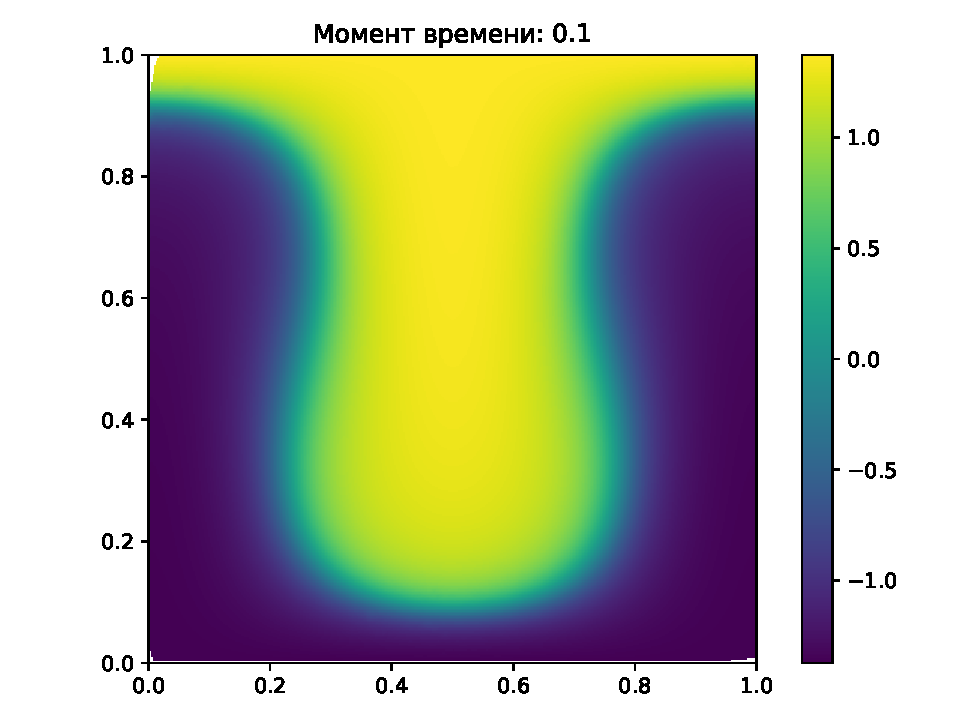
\includegraphics[width=8cm]{pictures/p5.pdf}
    \end{figure}
    \begin{figure}[H]
        \centering
        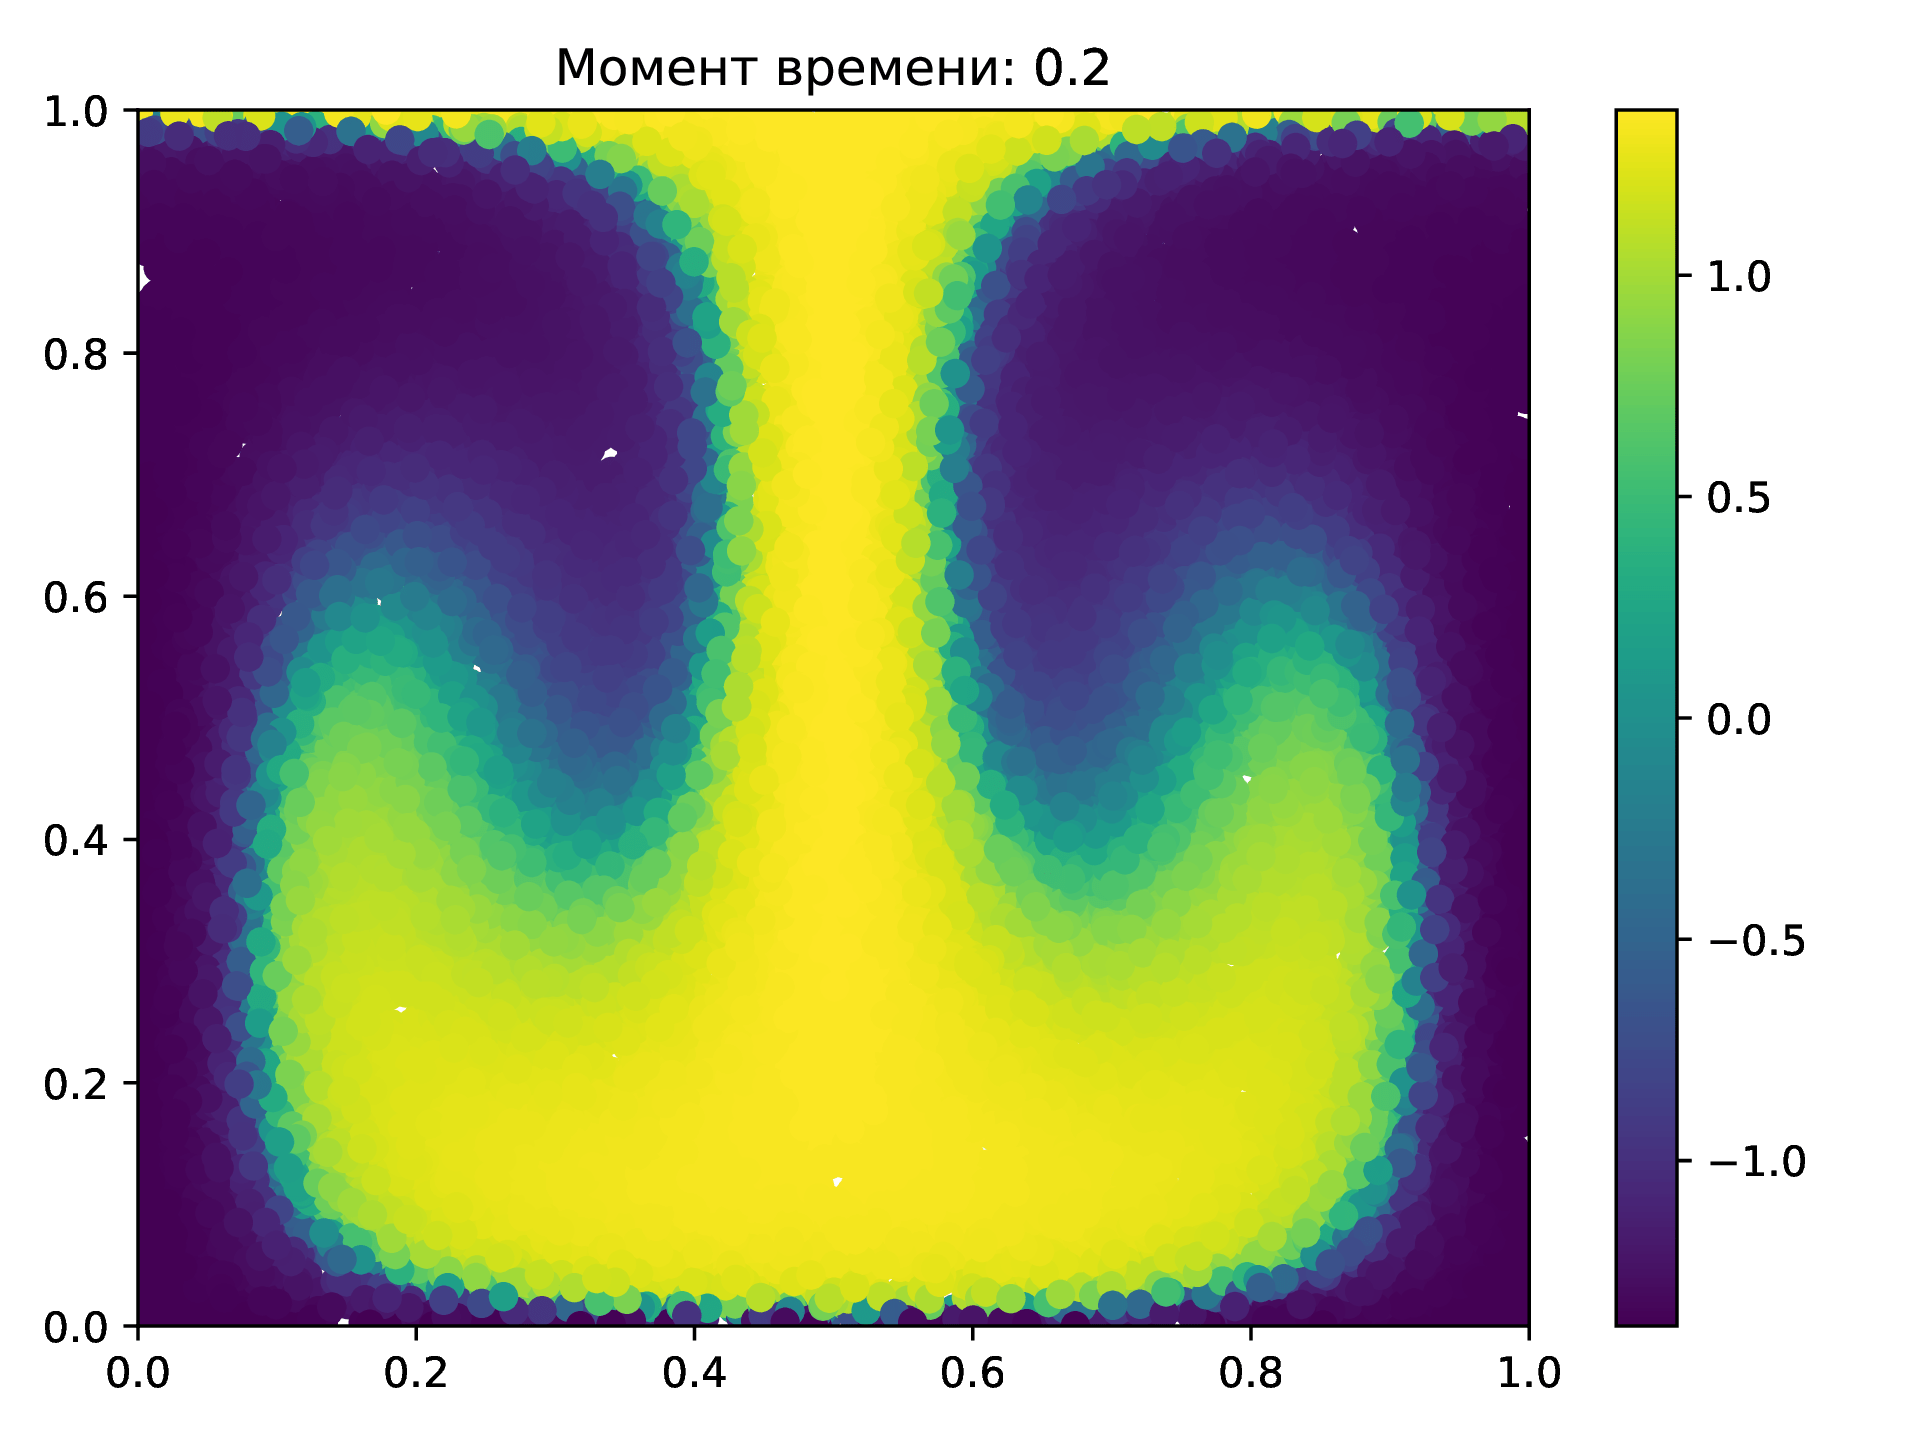
\includegraphics[width=8cm]{pictures/s10.png}
        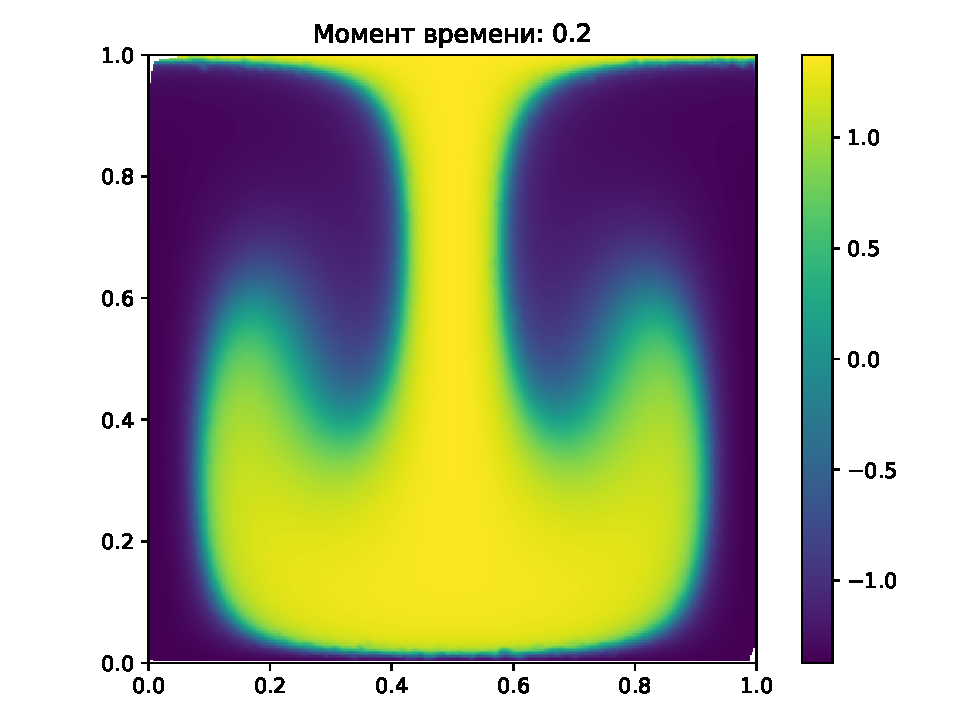
\includegraphics[width=8cm]{pictures/p10.pdf}
    \end{figure}
    \begin{figure}[H]
        \centering
        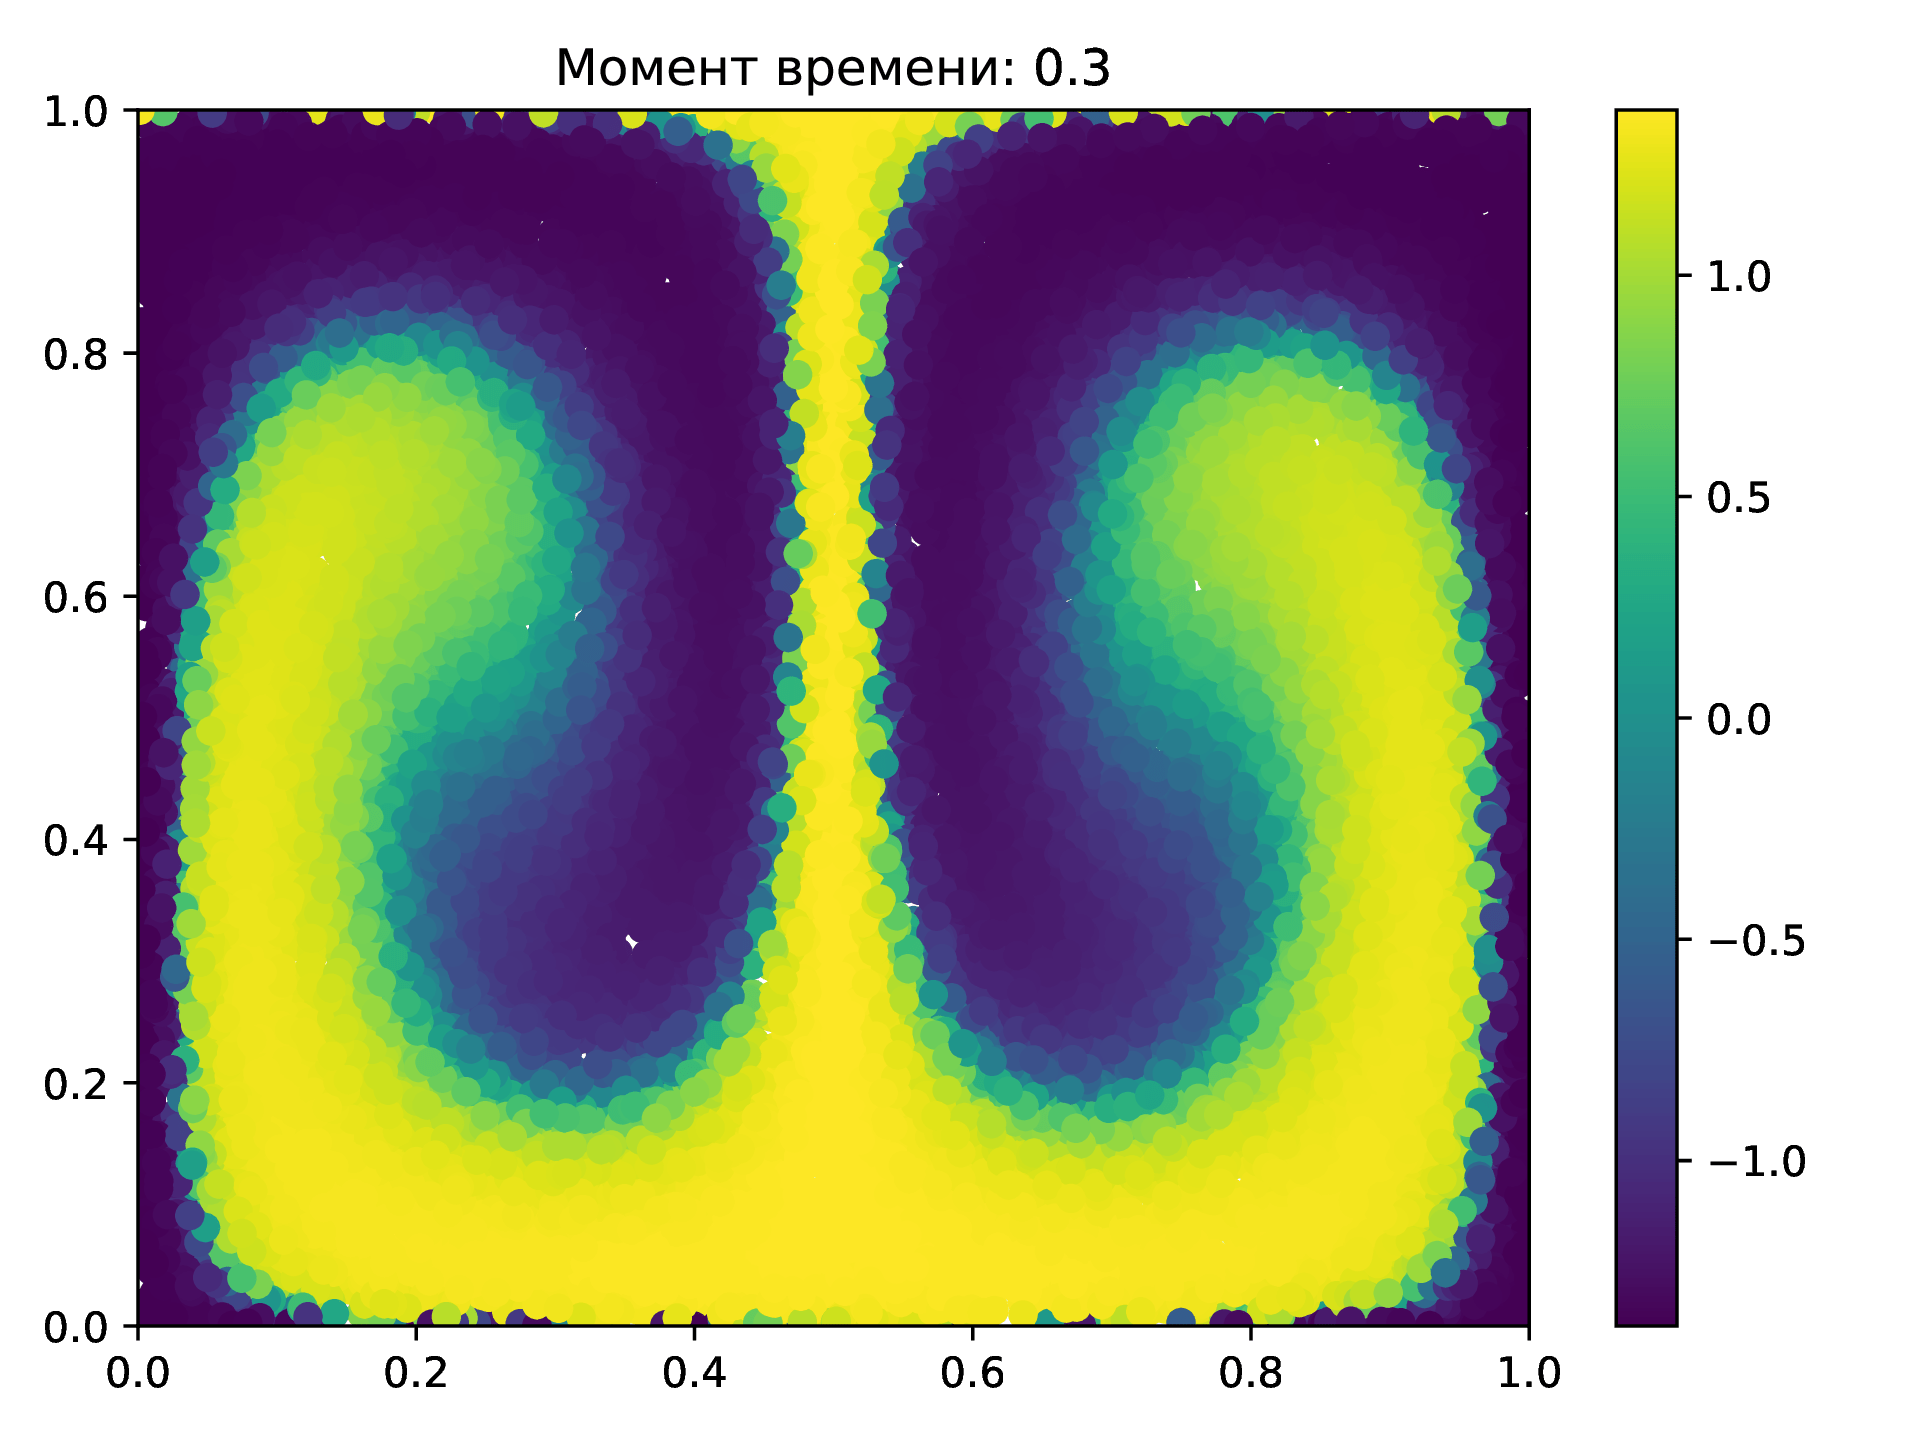
\includegraphics[width=8cm]{pictures/s15.png}
        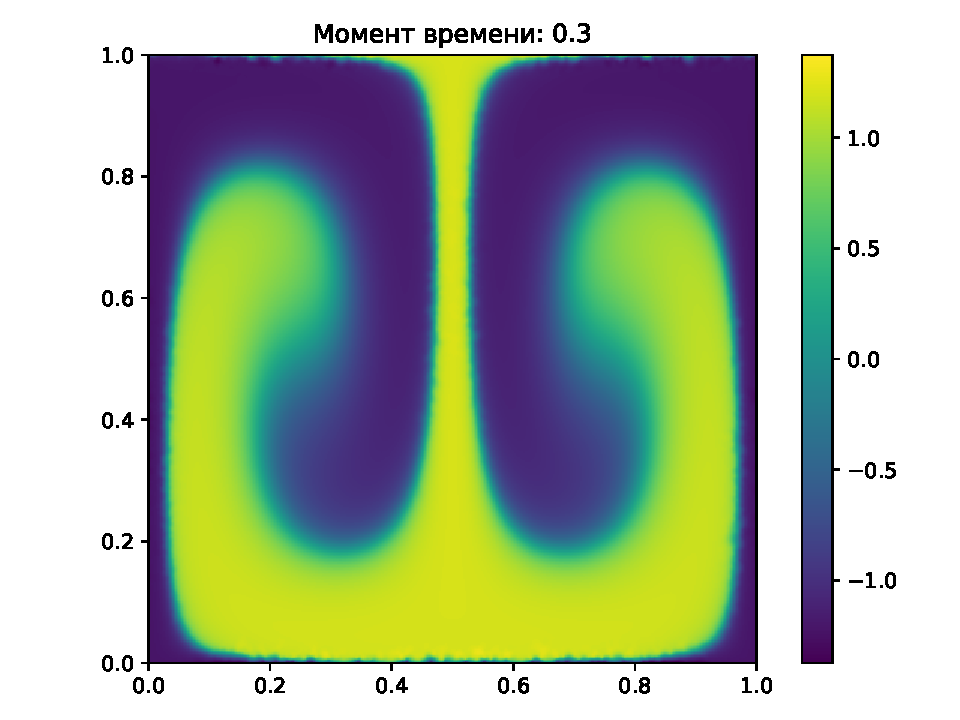
\includegraphics[width=8cm]{pictures/p15.pdf}
    \end{figure}
    \begin{figure}[H]
        \centering
        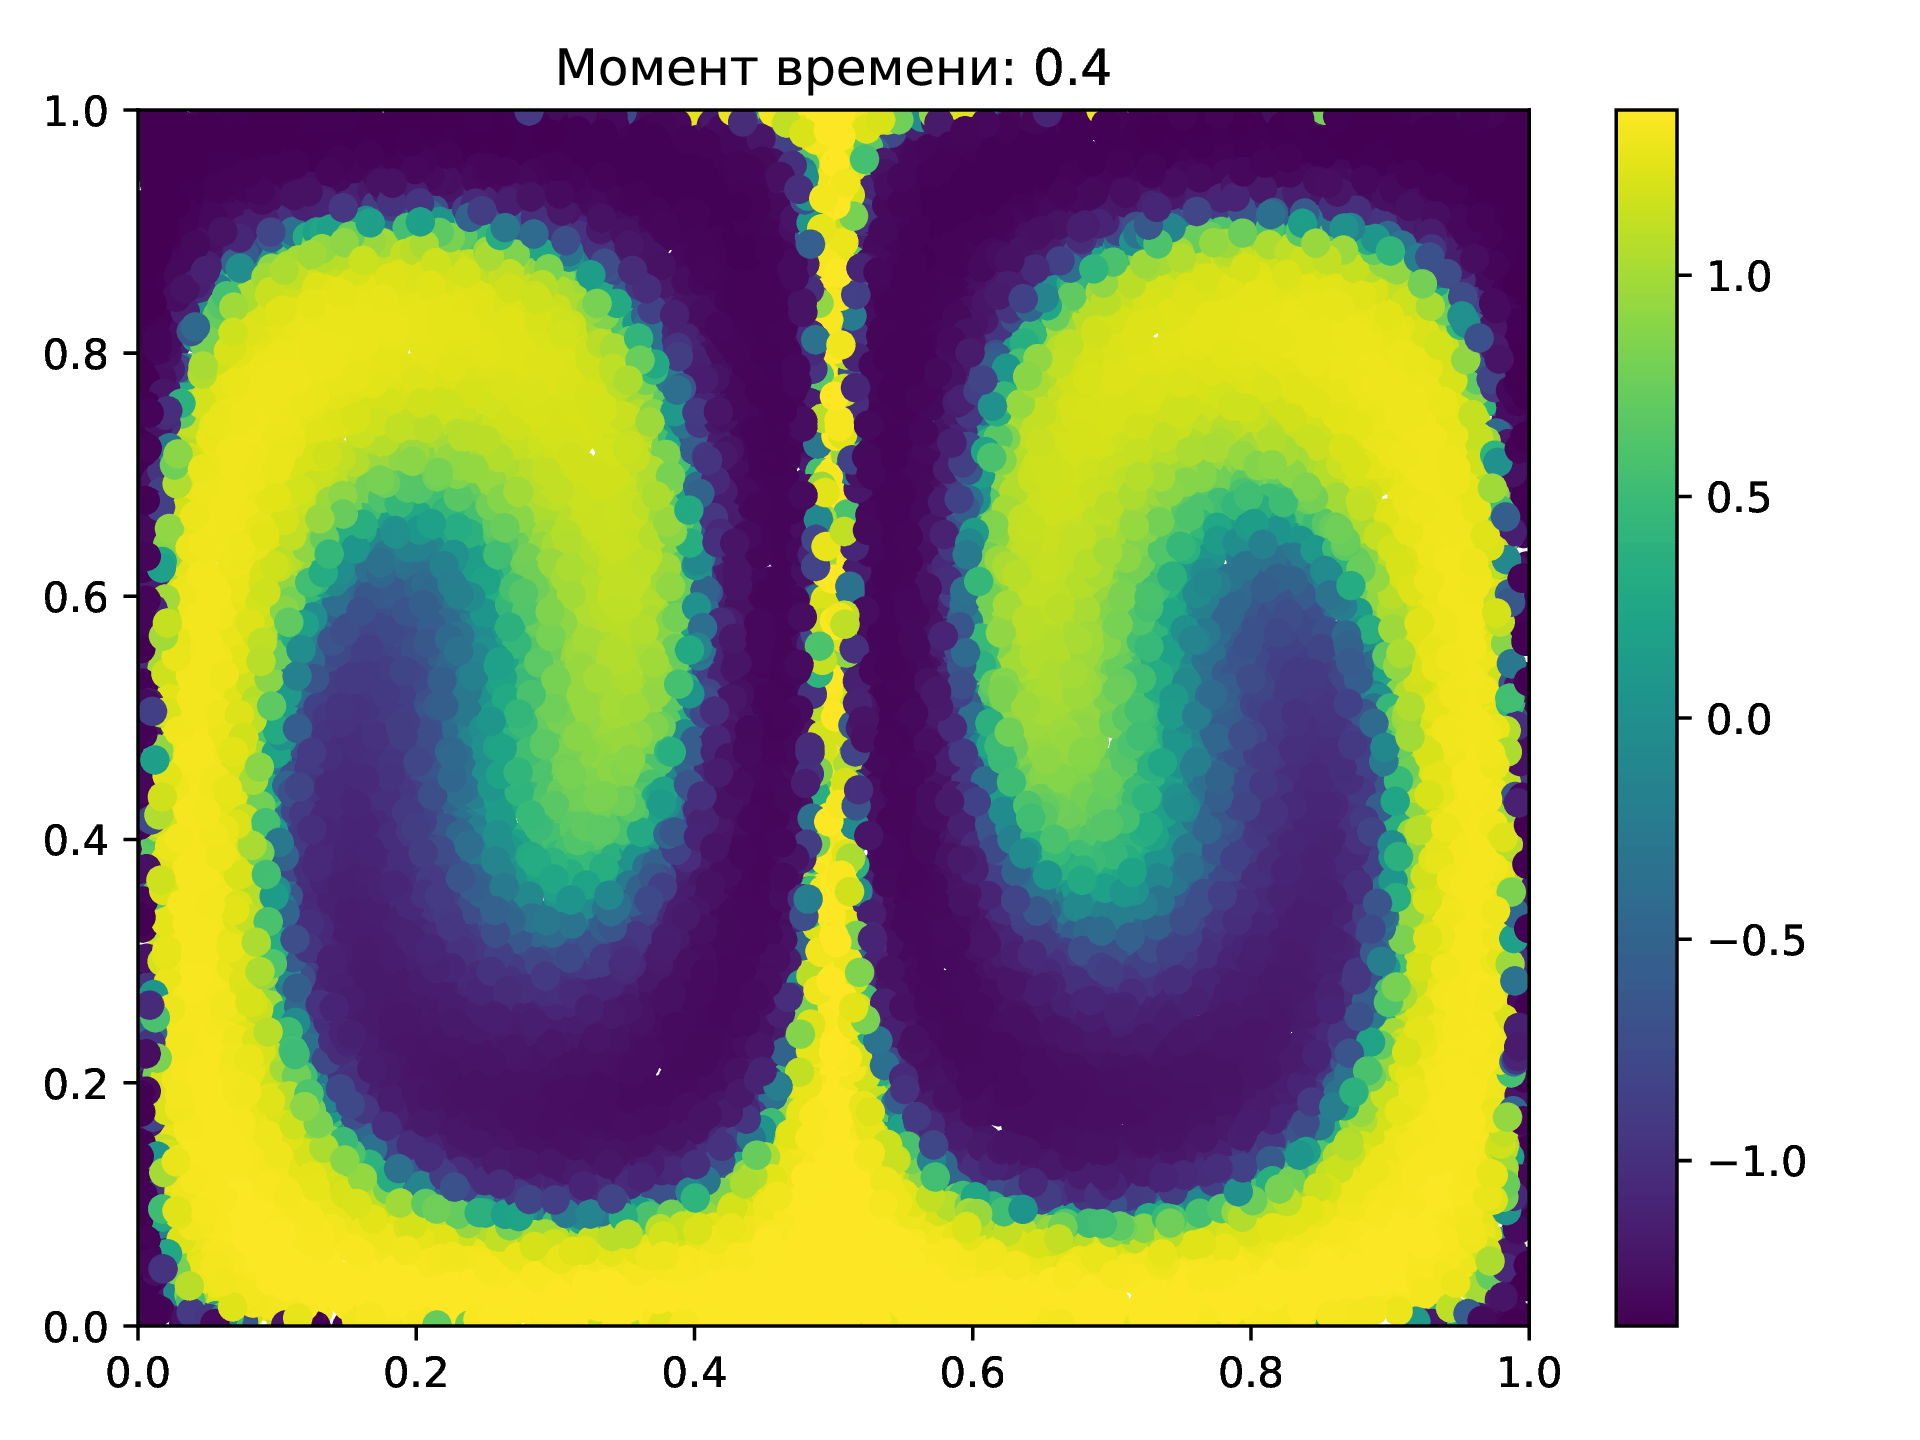
\includegraphics[width=8cm]{pictures/s20.png}
        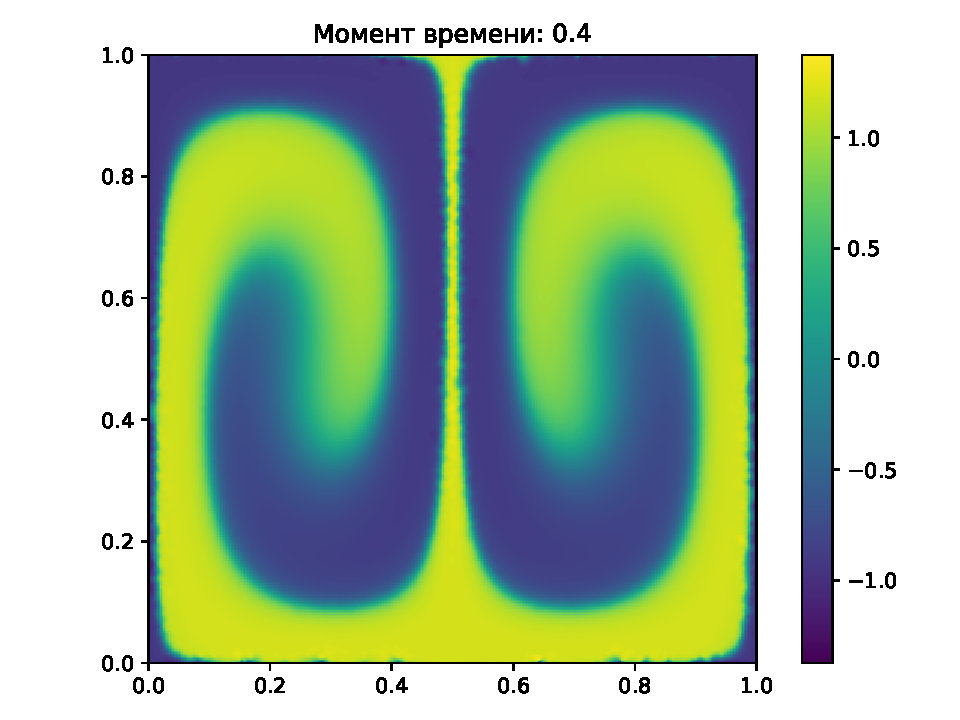
\includegraphics[width=8cm]{pictures/p20.pdf}
    \end{figure}


    \subsection{Турбулентность}
        В реальном мире очень сложно добиться идеальных условий где-либо, и для жидкостей и газов это явление называется турбулентностью. Для приближённого моделирования мы можем добавить некоторою случайную величину в дифференциальное уравнение, которая заставит частицу немного отклониться от траектории, заданной током.
        
        В этом эксперименте добавим слагаемым случайную величину из равномерного распределения на отрезке \( [-0.5, 0.5] \). 
    
        \begin{figure}[H]
            \centering
            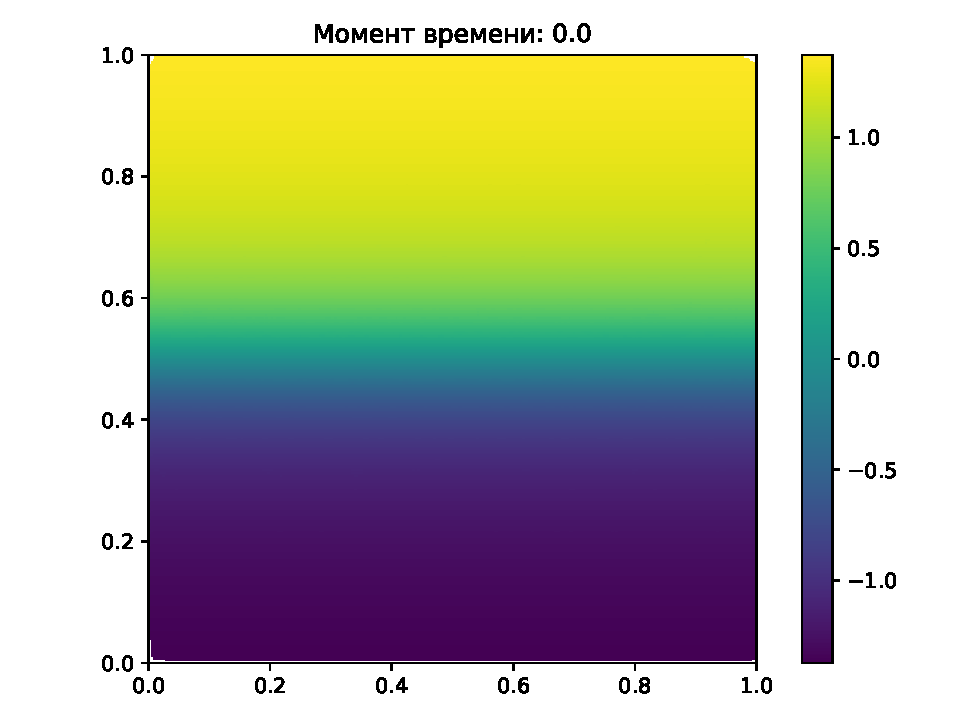
\includegraphics[width=8cm]{pictures/pr0.pdf}
            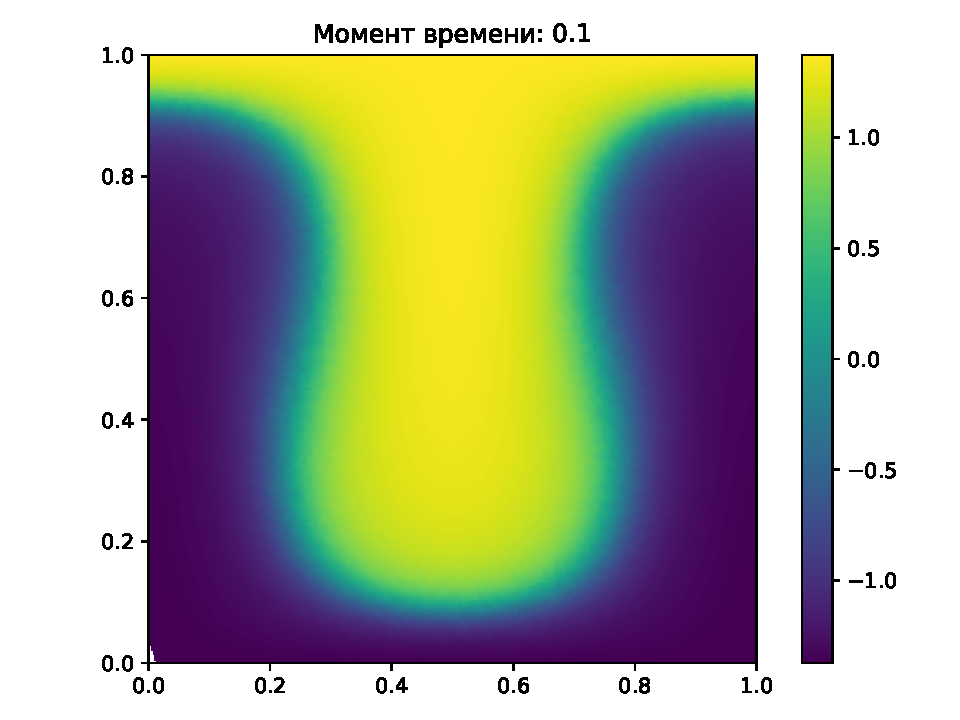
\includegraphics[width=8cm]{pictures/pr5.pdf}
        \end{figure}
        \begin{figure}[H]
            \centering
            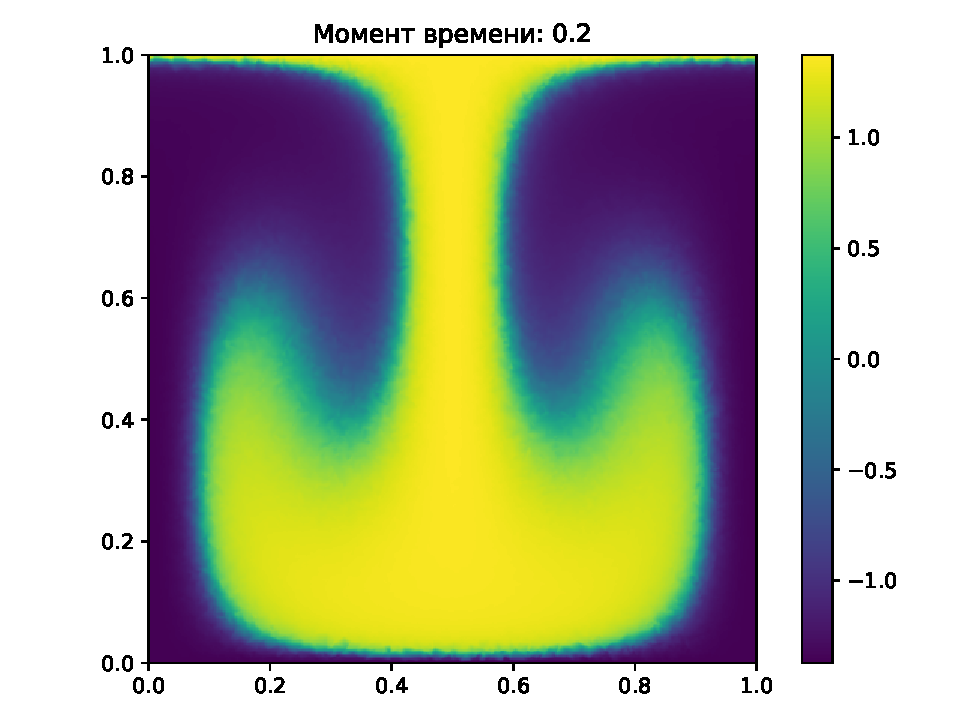
\includegraphics[width=8cm]{pictures/pr10.pdf}
            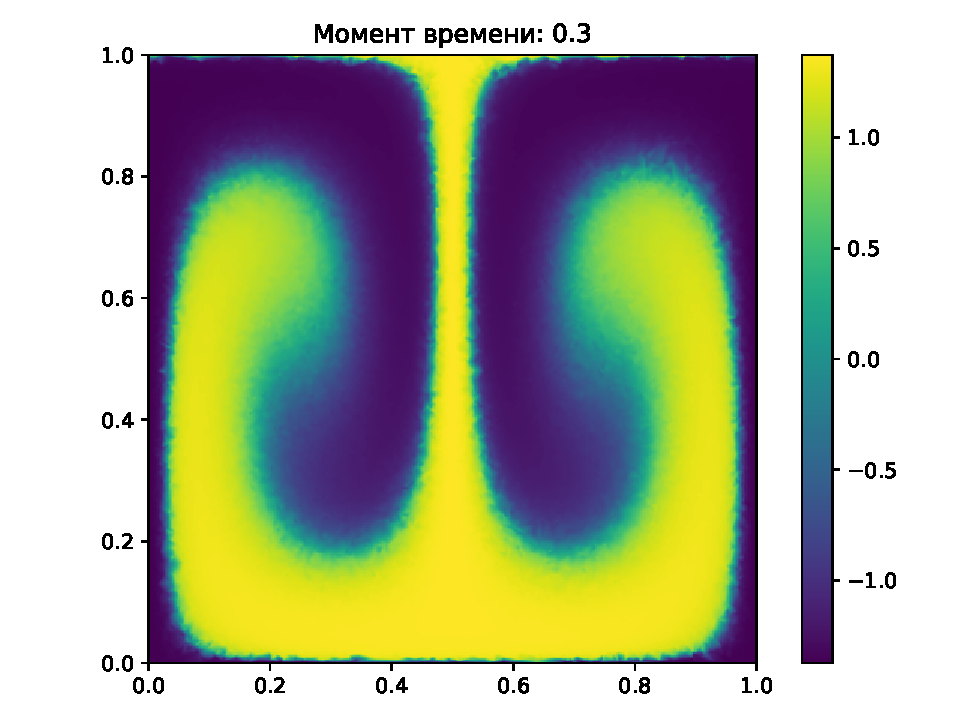
\includegraphics[width=8cm]{pictures/pr15.pdf}
        \end{figure}
        \begin{figure}[H]
            \centering
            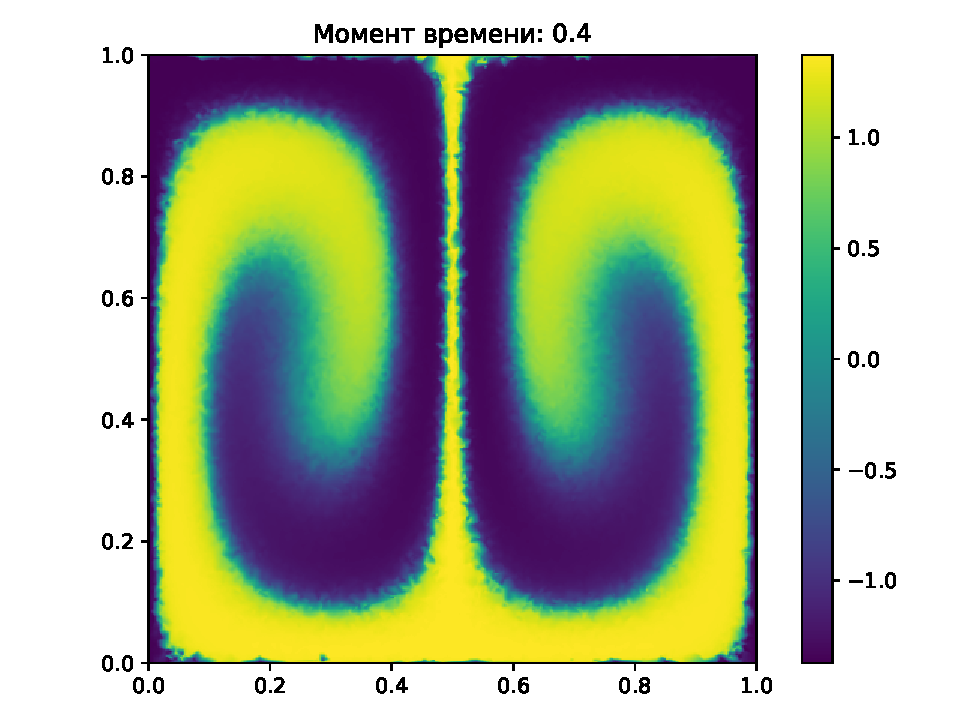
\includegraphics[width=8cm]{pictures/pr20.pdf}
        \end{figure}

        Видно, что в отличие от гладкого изображения идеальной модели здесь наблюдаются искажения из-за турбулентности.

        В эксперименте без турбулентности около границ можно было заметить эффект, который может напоминать турбулентность. Однако, это объясняется тем, что возле границ частиц находится меньшее количество и для интерполяции используются данные, которые находятся только с одной стороны от них.